\documentclass{article}
\usepackage{graphicx} % Required for inserting images
\usepackage{geometry}
\geometry{
    a4paper,
    left=2cm,
    right=2cm,
    top=2cm,
    bottom=2cm,
}

\newtheorem{theorem}{Theorem}
\usepackage{amsthm}
\usepackage{amsmath}
\usepackage{subcaption}

\title{Computer Vision HW5}
\author{Maxim Gluhovskoi}
\date{April 2024}


\begin{document}

\maketitle
\newpage
\section*{Problem 2: Theory Questions}

\subsection*{Q2.1}
\begin{flushleft}
    First we will prove that softmax is invariant to translation. We want to show that: 
    $softmax(x)=softmax(x+c)$ for every c within the reals. We know that for each index i in a vertex x 
    softmax is defined as follows: $softamx(x_i)=\frac{e^{x_i}}{\sum_{j}e^{x_j}}$. \\
    Let x be some arbitrarly large vector then if we add an arbitrary c to each $x_i$ within x we 
    get $softmax(x_i+c)=\frac{e^{x_i+c}}{\sum_{j}e^{x_j+c}}=\frac{e^{x_i}e^{c}}{\sum_{j}e^{x_j}e^{c}}
    =\frac{e^{x_i}e^{c}}{e^{c}\sum_{j}e^{x_j}}=\frac{e^{x_i}}{\sum_{j}e^{x_j}}$ as desired. Therefore 
    we have proven that softmax is invariant to translation.\\
    Now lets show why using $c=-max(x_i)$ is a good idea. If our $c=0$ then our max $x_i$ value could 
    be quite large resulting in stability, overflow, and more difficult computation. On the other 
    hand if we somewhat normalize our $x_i$ values by setting the max to 0 we will limit our 
    exponentials to be less than 1 fixing our instability issues and potential overflow. This also 
    keeps the results the same since we previously proved that softmax is invariant to translation.

\end{flushleft}
\subsection*{Q2.2}
\begin{flushleft}
    a) Softmax has a range of 0 to 1 and the sum over all elements is 1 since we 
    are doing the following $\sum_{i}(\frac{e^{x_i}}{\sum_{j}(e^{x_j})})=
    \frac{\sum_{i}e^{x_i}}{\sum_{j}e^{x_j}}=1$.\\
    b) Probability distribution.\\
    c) The first step: $s_i=e^{x_i}$ takes the individual value/probability. The exponent 
    eleminates any negative values and results in larger differences in resulting values resulting 
    in better differentiation between values and better training. The second step: $S=\sum(s_i)$ 
    takes the total probability value and will act as a normalizer for each $s_i$ to make the output
    values range from 0 to 1. The third steps: $\frac{s_i}{S}$ applies the normalizer resulting in 
    a clean looking probability value of $s_i$.
\end{flushleft}
\subsection*{Q2.3}
\begin{flushleft}
    First I will show the individual scalar derivatives of W, x, and b. We are given the formula: 
    $y_j=\sum_{i=1}^{d}x_iW_{ij}+b_j$ so the derivative: $\frac{dj}{dw_{ij}}=
    \frac{dj}{dy}\frac{dy}{dw_{ij}}=\frac{dj}{dy}*x_i$ and $\frac{dj}{dx_{i}}=
    \frac{dj}{dy}\frac{dy}{dx_{i}}=\frac{dj}{dy}*\sum_{i=1}^{k}w_{ij}$ and 
    $\frac{dj}{b_j}=\frac{dj}{dy}\frac{dy}{dw_j}=\frac{dj}{dy}*1$. Re-forming these into 
    matrix form we get $\frac{\partial J}{\partial W}=
    \frac{\partial J}{\partial y}\frac{\partial y}{\partial W}=
    x (\frac{\partial J}{\partial y})^T$ and 
    $\frac{\partial J}{\partial x}=
    \frac{\partial J}{\partial y}\frac{\partial y}{\partial x}=
    W \frac{\partial J}{\partial y}$ and
    $\frac{\partial J}{\partial b}=
    \frac{\partial J}{\partial y}\frac{\partial y}{\partial b}=
    \frac{\partial J}{\partial y}*1$.
\end{flushleft}
\subsection*{Q2.4}
    
\begin{flushleft}
    part 1) 
    $[w_0 w_1 w_2 w_3 w_4 w_5 w_6 w_7 w_8]$
    $\begin{bmatrix}
        0 & 0 & 0 & 0 & x_0 & x_1&0&x_3&x_4\\
        0&0&0&x_0&x_1&x_2&x_3&x_4&x_5\\
        0&0&0&x_1&x_2&0&x_4&x_5&0\\
        0&x_0&x_1&0&x_3&x_4&0&x_6&x_7\\
        x_0&x_1&x_2&x_3&x_4&x_5&x_6&x_7&x_8\\
        x_1&x_2&0&x_4&x_5&0&x_7&x_8&0\\
        0&x_3&x_4&0&x_6&x_7&0&0&0\\
        x_3&x_4&x_5&x_6&x_7&x_8&0&0&0\\
        x_4&x_5&0&x_7&x_8&0&0&0&0
    \end{bmatrix}$
    \\
    part 2) The size of the first matrix representing the kernels is 64by25 and the second is 
    25by3136 so our resulting matrix is 64by3136 which is then reshaped to 64by56by56.
\end{flushleft}
\newpage
\subsection*{Q3.1.1}
\begin{flushleft}
    Initializing a network to all zeros would result in an output of all zeros making it extremely hard 
    to impossible to do further training if most layers are relu or other activation functions where f(0)=0.
    This may also result in symmetry between neurons since all of the neurons will have the same gradient 
    resulting in lots of neurons doing the same thing making the neural network inefficient.
\end{flushleft}
\subsection*{Q3.1.3}
\begin{flushleft}
    We initialize with random numbers so that our gradients will be random and 
    result in different patterns being learned (breaking symmetry and reducing 
    redundant neurons). We scale the initialization 
    depending on layer size since we want the variance between layers to be the 
    same in regards to the layer size this will help prevent exploding and vanishing 
    gradients through the multiplicative effect that gradients undergo in deep 
    networks.
\end{flushleft}
\newpage
\subsection*{Q4.2}
\begin{figure}[htbp]
    \centering
    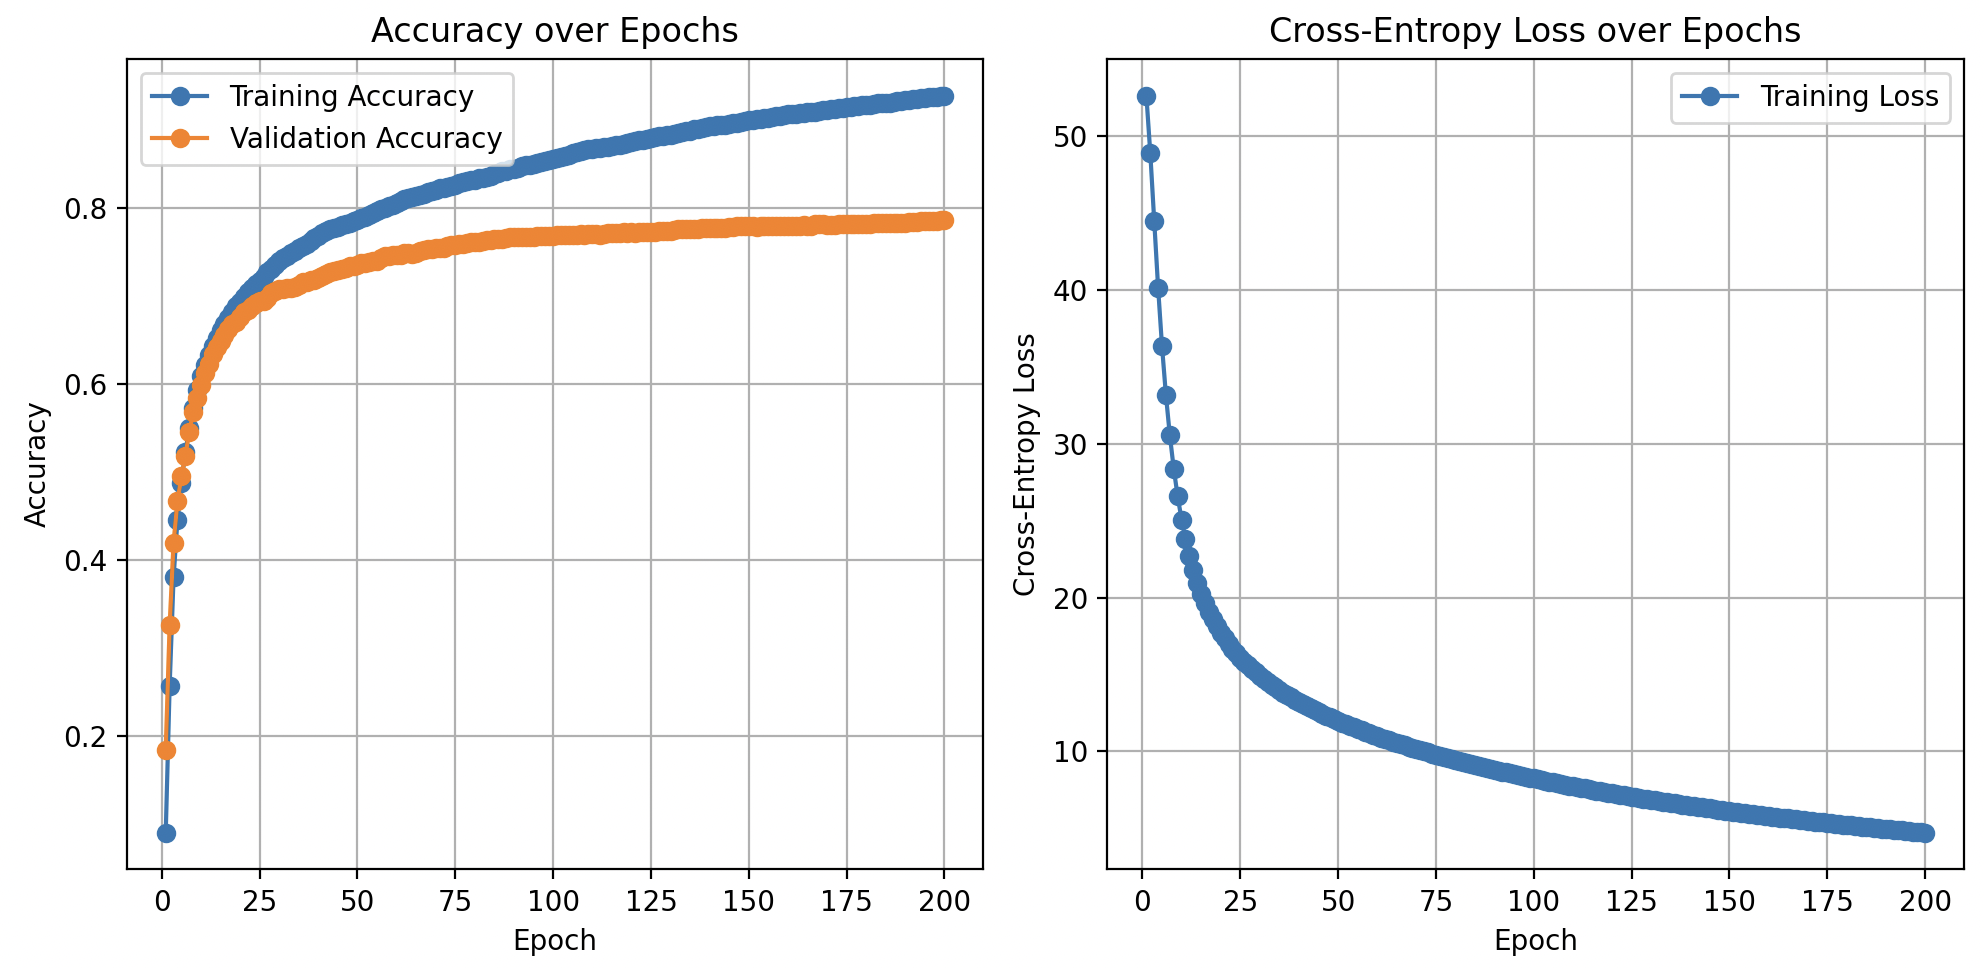
\includegraphics[width=0.4\linewidth]{best_lr.png}
    \caption{best learning rate}
  \end{figure}
  
  \begin{figure}[htbp]
    \centering
    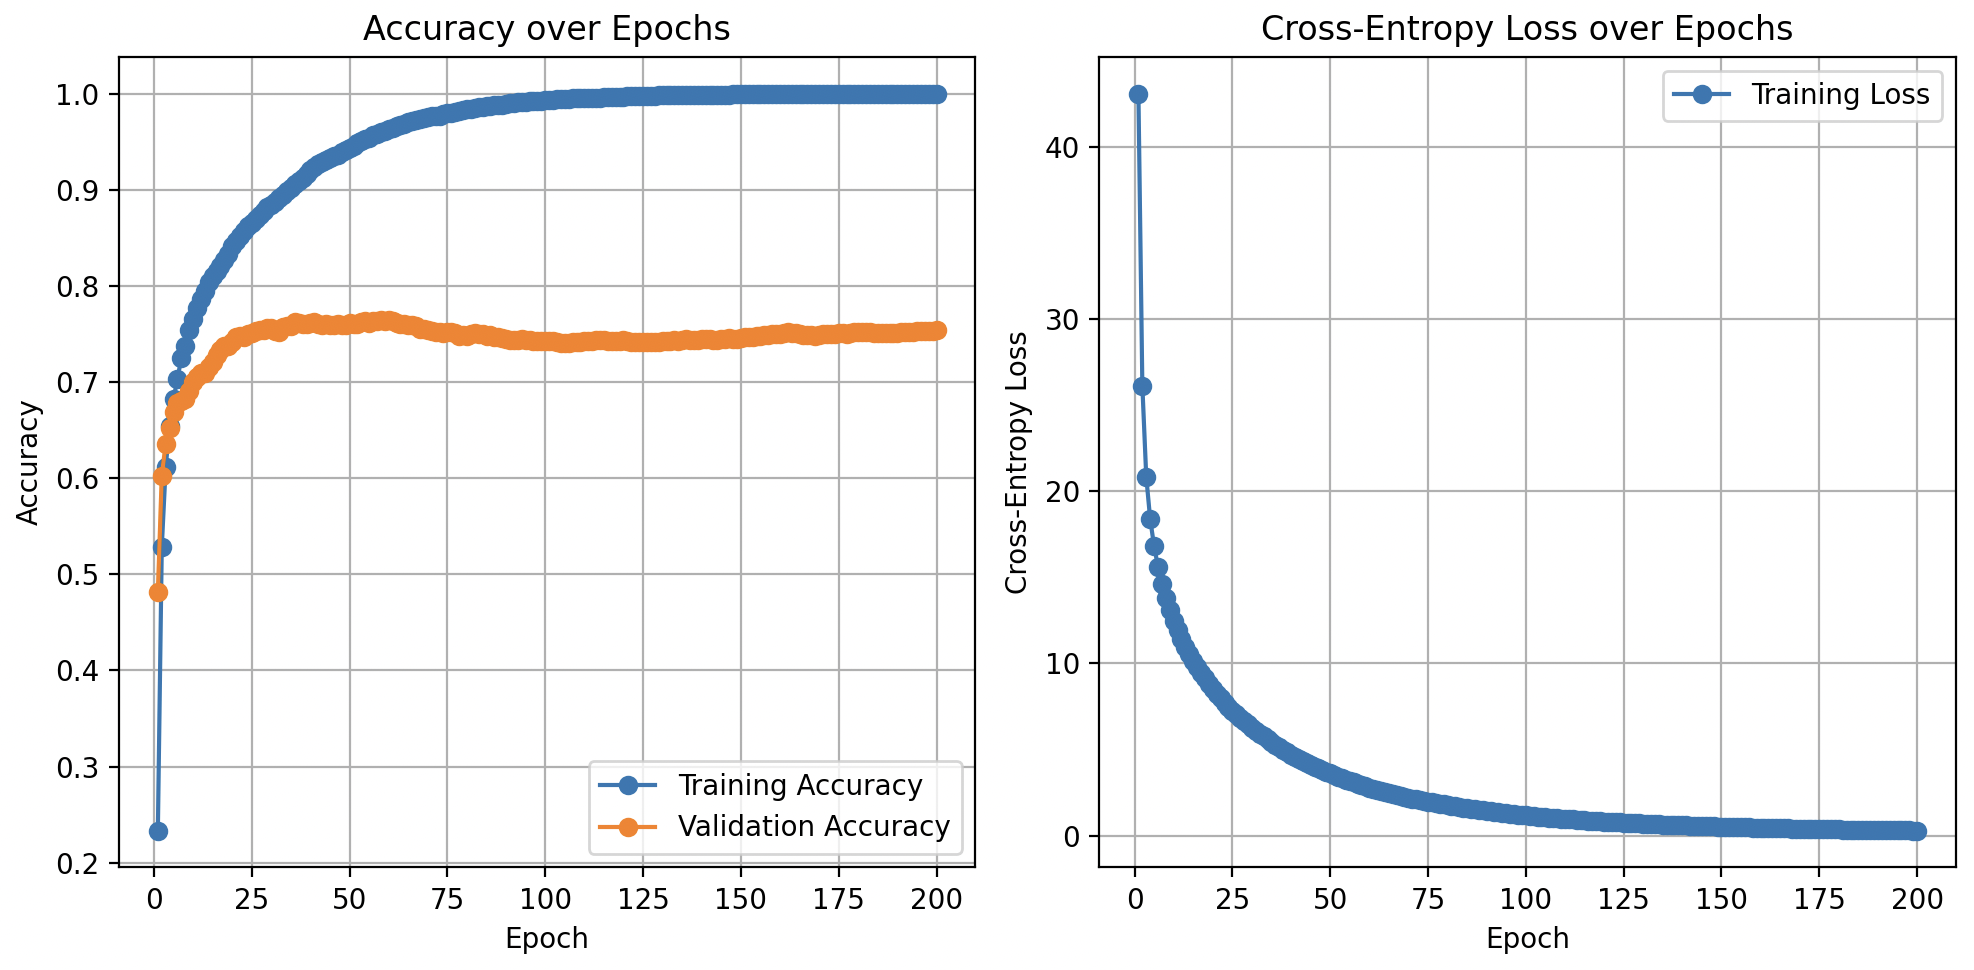
\includegraphics[width=0.4\linewidth]{10x_lr.png}
    \caption{10x learning rate}
  \end{figure}
  
  \begin{figure}[htbp]
    \centering
    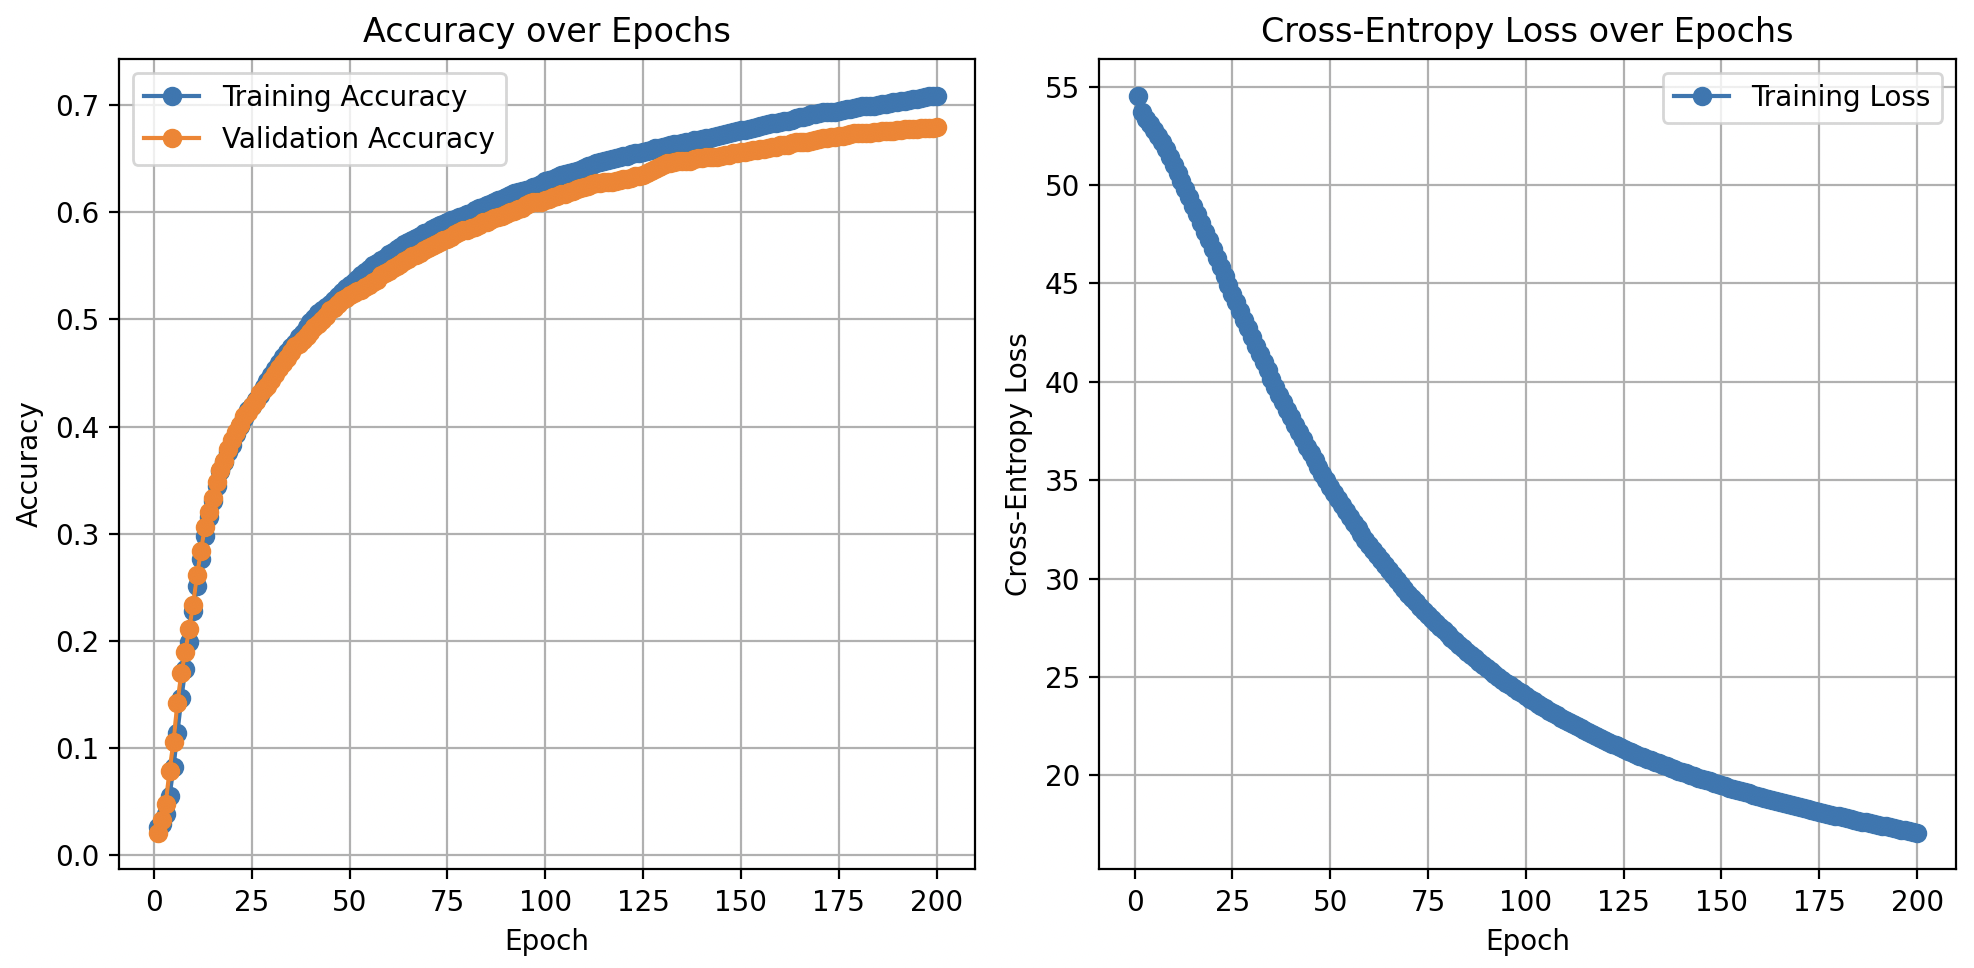
\includegraphics[width=0.4\linewidth]{tenth_lr.png}
    \caption{1/10th learning rate}
  \end{figure}
  Higher learning rates result in faster optimization of training accuracy,
  but validation accuracy suffers greatly since we are over training. Meanwhile,
  lower learning rates result in slower optimization of training accuracy,
  but we are not overtraining as much so our validation accuracy stays much closer 
  to our training accuracy. My best learning rate was 1e-3 with 200 epochs and batch 
  size 15. My best validation accuracy was 78.67\%.
\newpage
\subsection*{Q4.3}
\begin{figure}[htbp]
    \centering
    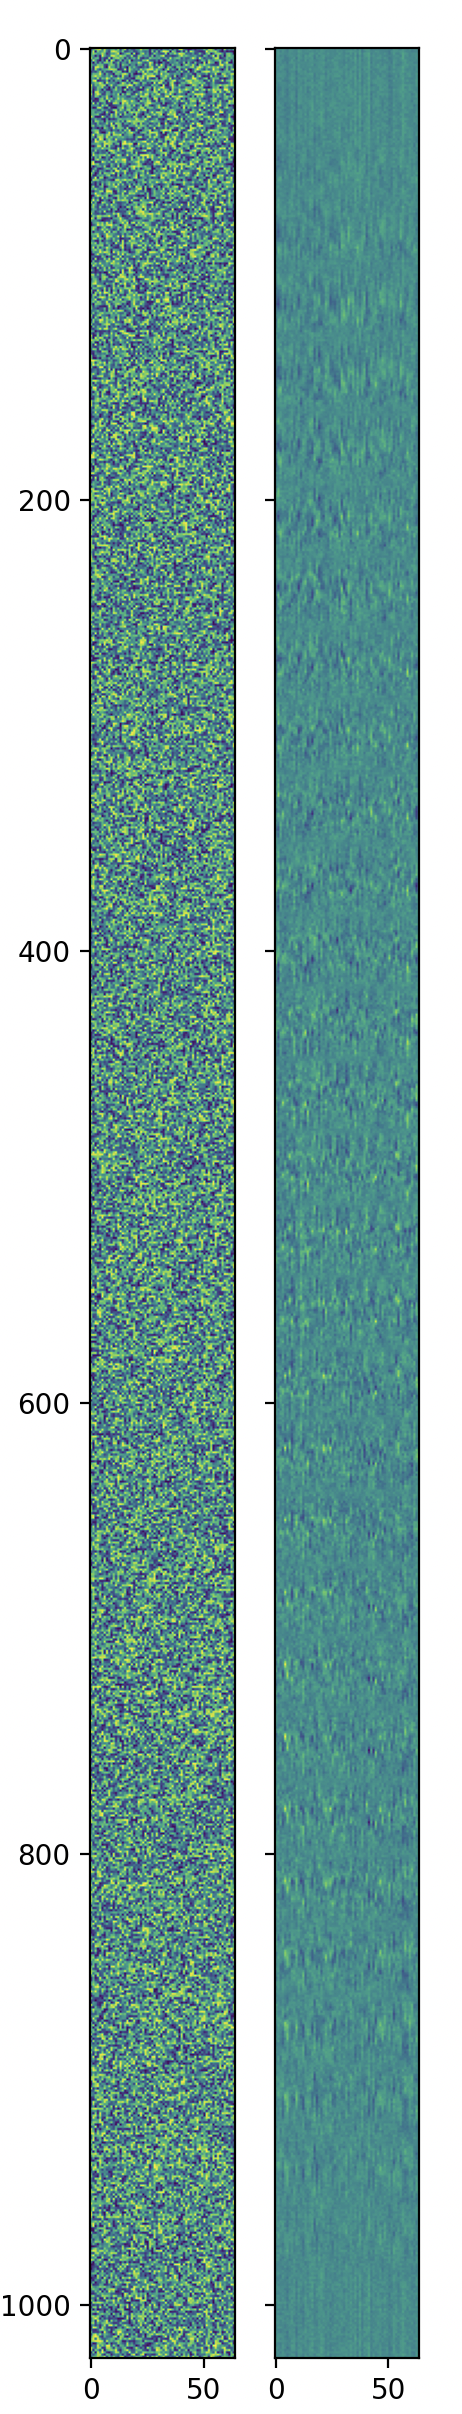
\includegraphics[width=0.2\linewidth]{weights_rep.png}
    \caption{1st layer weights init (left) trained (right)}
  \end{figure}
  The learned weights develop streaking lines downwards. These patches repeat every 
  36 or so rows corresponding to the rows of the input images. It basically changes 
  from streaks to just blur and repeats.
\newpage
\subsection*{Q4.4}
\begin{figure}[htbp]
    \centering
    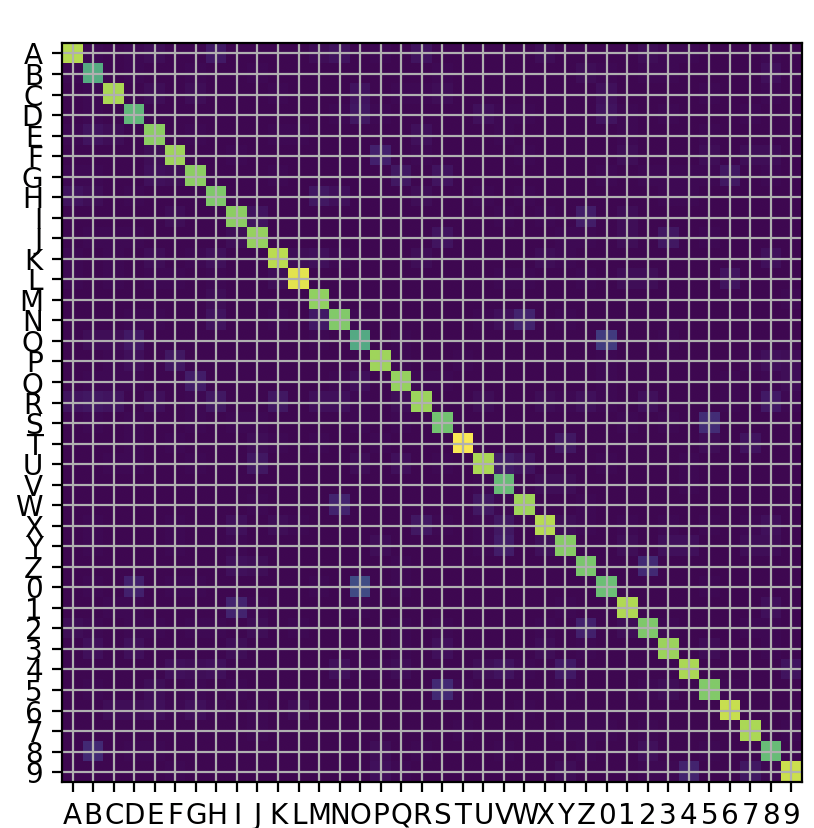
\includegraphics[width=0.9\linewidth]{confusion_matrix.png}
    \caption{confusion matrix}
  \end{figure}
\begin{flushleft}
    Some of the pairs that the algoirthm is getting cofused on for example include:
    0 and O, 5 and S, and B and 8. These all look pretty similiar to each other so it makes 
    sense that the network occasionally gets these wrong/mismatched.
\end{flushleft}
\newpage
\subsection*{Q4 EXTRA}
\begin{flushleft}
    for fun I tried making the neural network as good as possible and ended up getting 86.44\% 
    accuracy with a total of 4 layers. Details can be found in the code. I include some charts 
    about the model and the confusion matrix for this model.
\end{flushleft}
\begin{figure}[htbp]
    \centering
    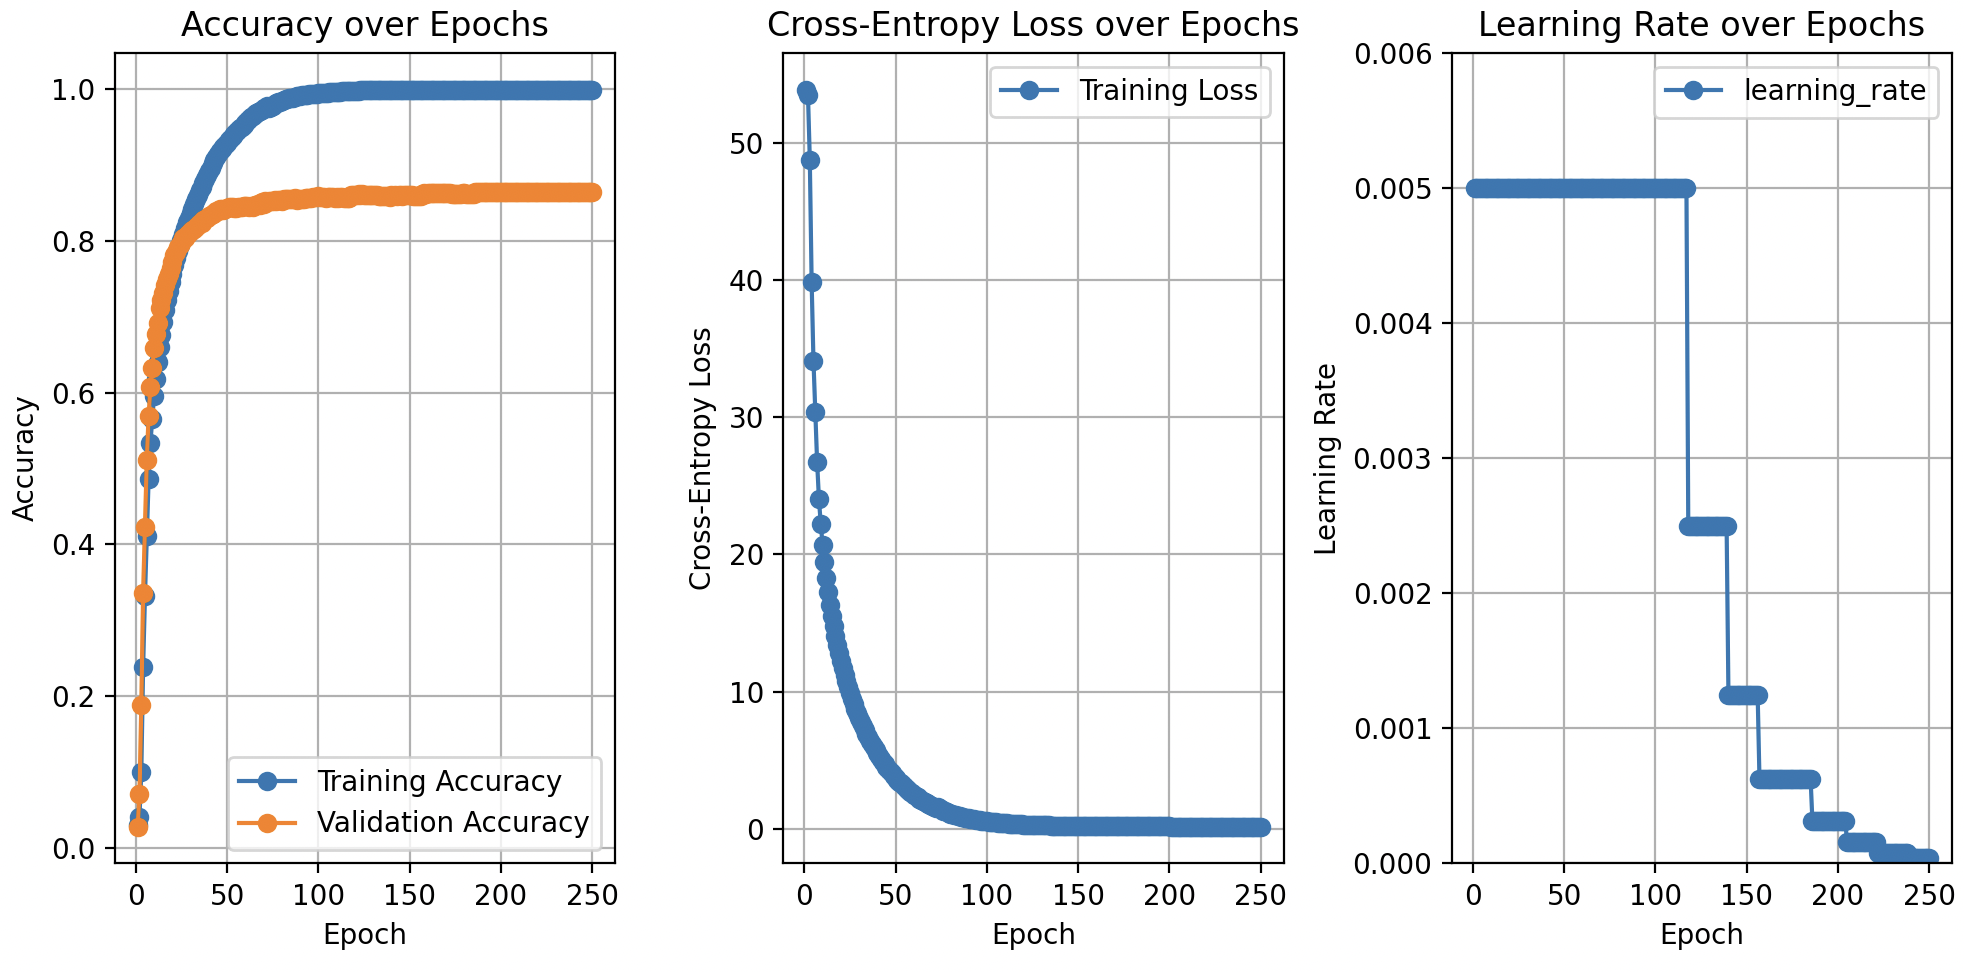
\includegraphics[width=0.9\linewidth]{extra_model_data.png}
  \end{figure}
  \begin{figure}[htbp]
    \centering
    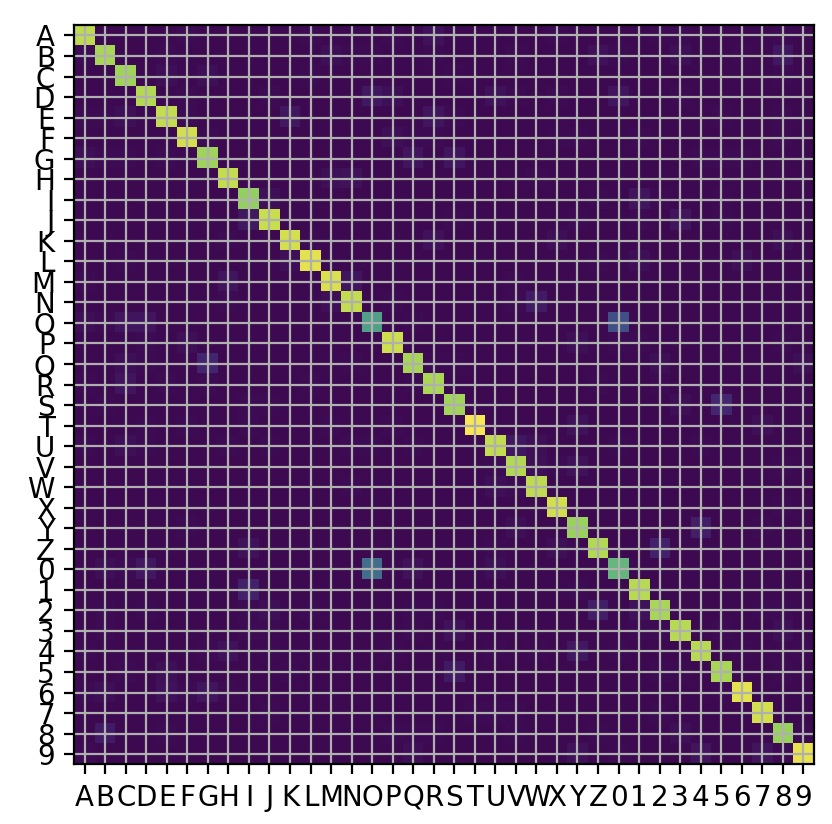
\includegraphics[width=0.6\linewidth]{extra_conf_mat.png}
  \end{figure}


\newpage
\subsection*{Q5.1}
\begin{flushleft}
    The method outlined in the writeup assumes that each letter/number is 32 by 32 pixels in size.
    If it is not in this size then it might provide wrong letters or skip over letters. It is also assuming that 
    we are not using anything except for letters and numbers so any punctuation will result in miss labeled 
    data. Here are some example images that may fail:
\end{flushleft}
    \begin{figure}[htbp]
    \centering
    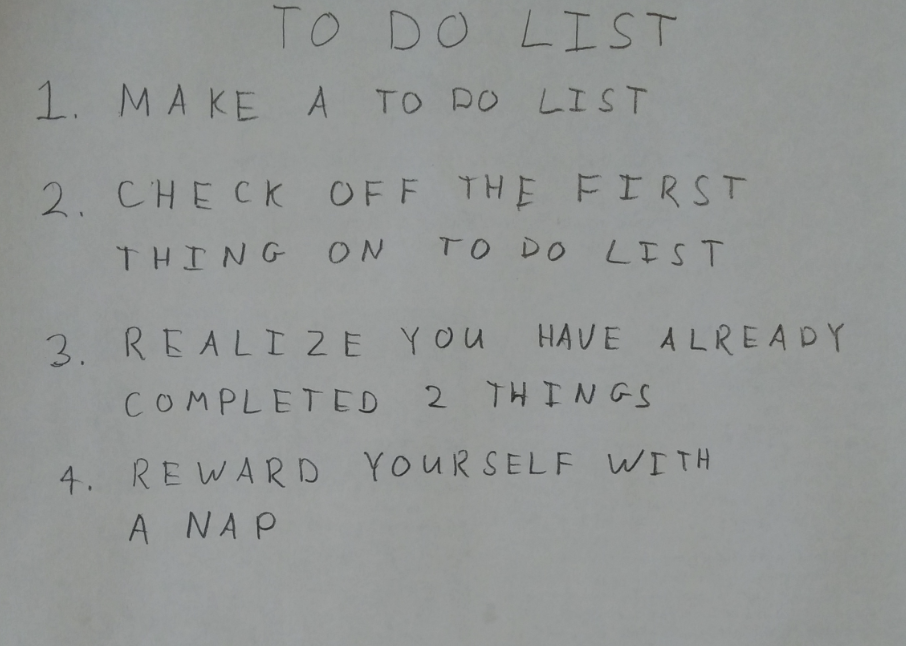
\includegraphics[width=0.4\linewidth]{punctuation.png}
    \caption{punctuation results in non-letter characters being labeled}
  \end{figure}
  \begin{figure}[htbp]
    \centering
    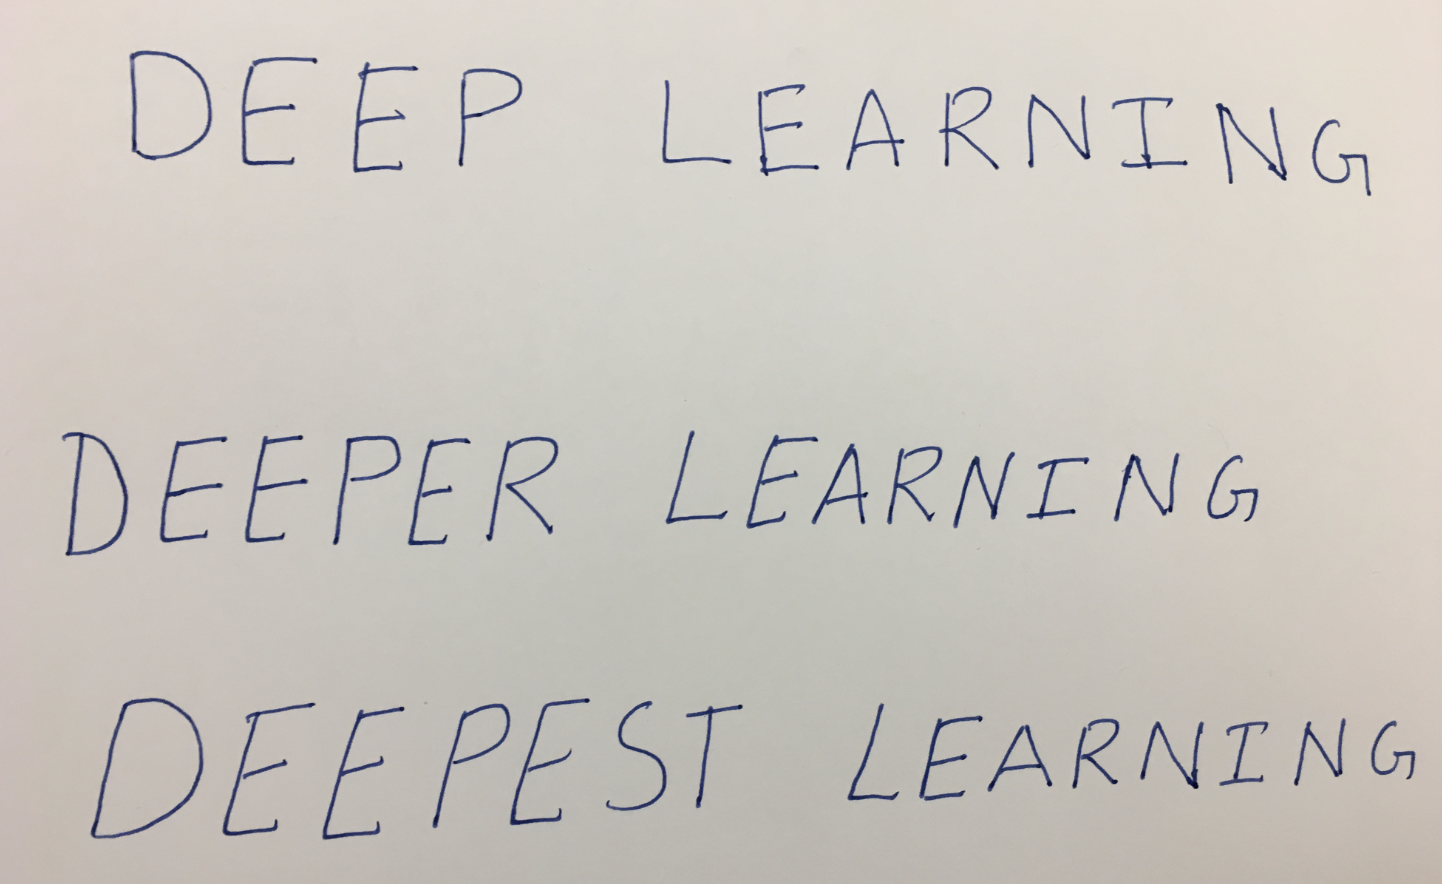
\includegraphics[width=0.4\linewidth]{close.png}
    \caption{Letters beign too small or too big can result in skipped or added letters}
  \end{figure}
\newpage
\subsection*{Q5.3}
\begin{figure}
    \centering
    \begin{subfigure}[h]{0.4\textwidth}
        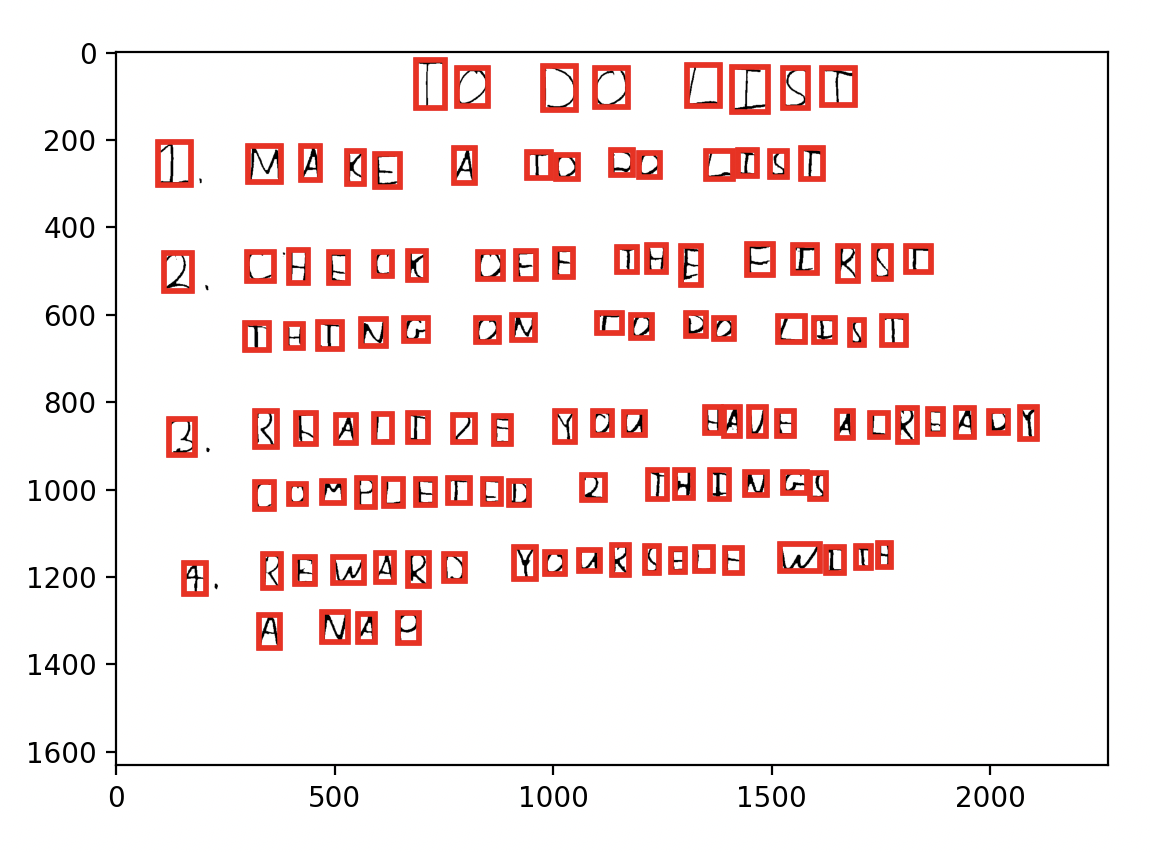
\includegraphics[width=\textwidth]{box1.png}
    \end{subfigure}
    \hfill
    \begin{subfigure}[h]{0.4\textwidth}
        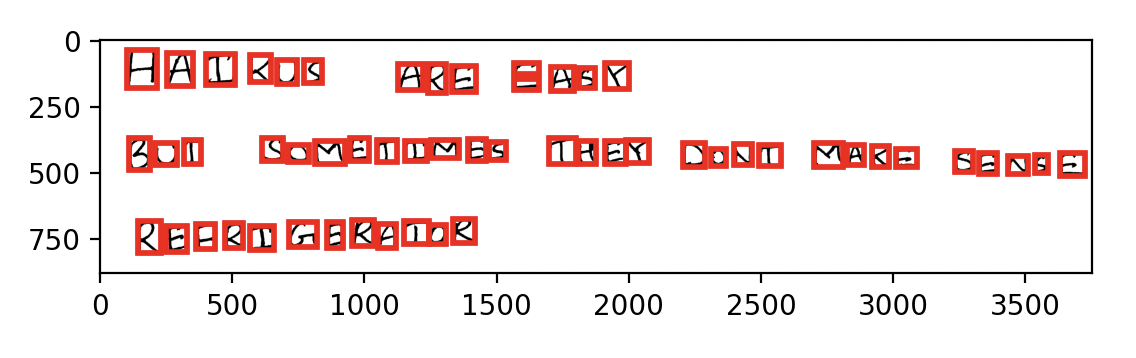
\includegraphics[width=\textwidth]{box2.png}
    \end{subfigure}
\end{figure}

\begin{figure}
    \centering
    \begin{subfigure}[h]{0.4\textwidth}
        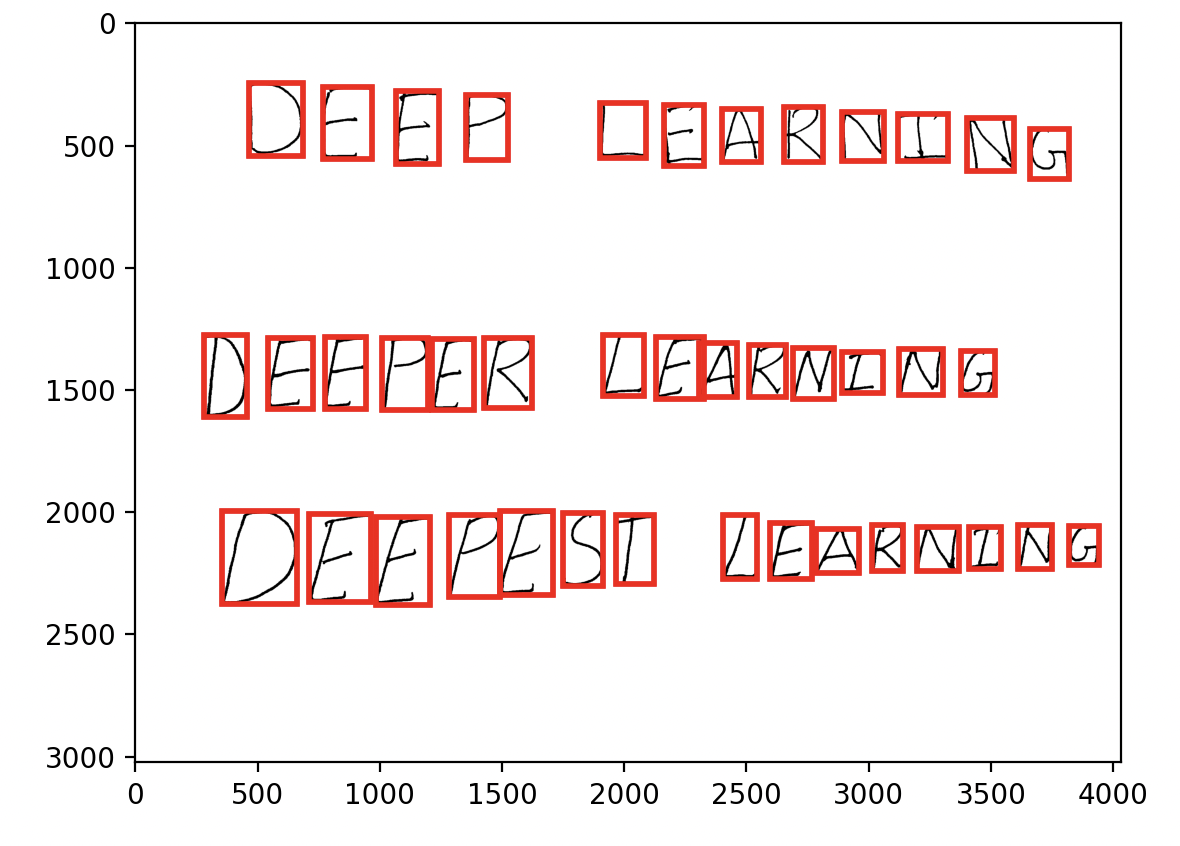
\includegraphics[width=\textwidth]{box3.png}
    \end{subfigure}
    \hfill
    \begin{subfigure}[h]{0.4\textwidth}
        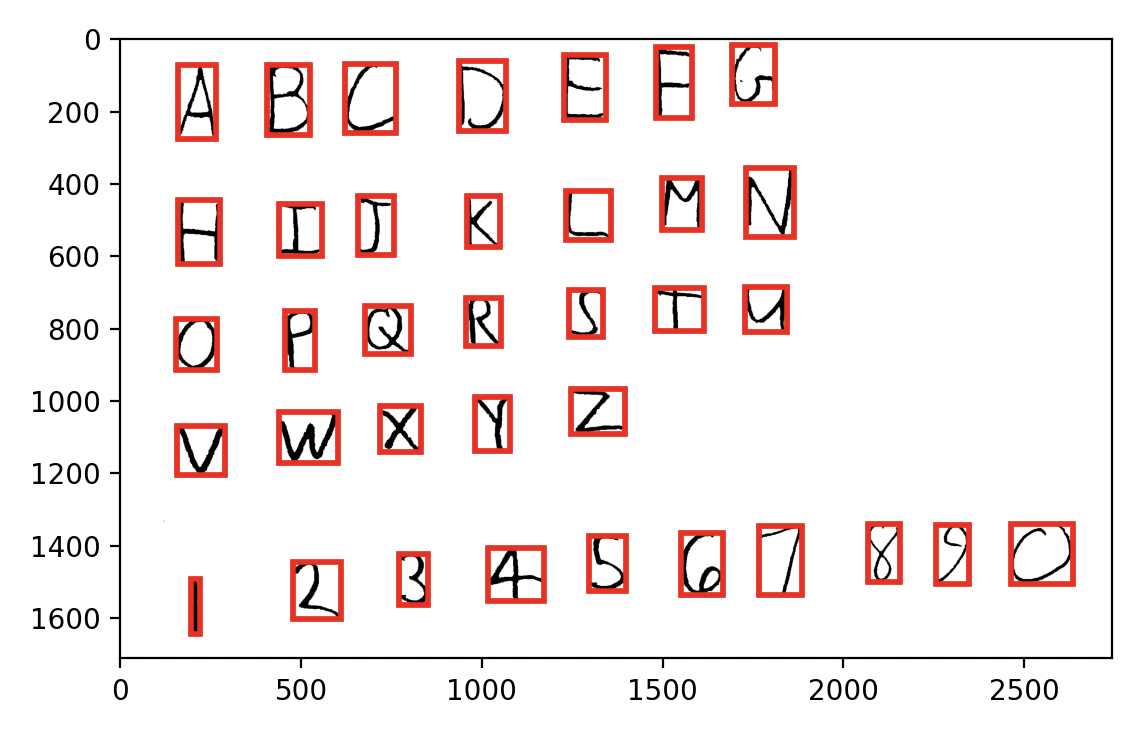
\includegraphics[width=\textwidth]{box4.png}
    \end{subfigure}
\end{figure}
\newpage
\subsection*{Q5.4}

I did some post processing to fix some of the common errors with 0 and O and B and 8 and 5 and S by checking if there 
are letters in front or behind and if so switching the number for a letter.\\
Here are my results for that:\\
\begin{figure}[htbp]
    \centering
    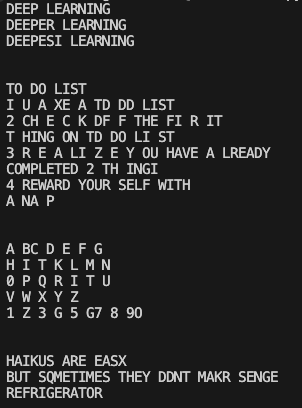
\includegraphics[width=0.6\linewidth]{final_res1.png}
\end{figure}
\newpage
Without the post processing I get:
\begin{figure}[htbp]
    \centering
    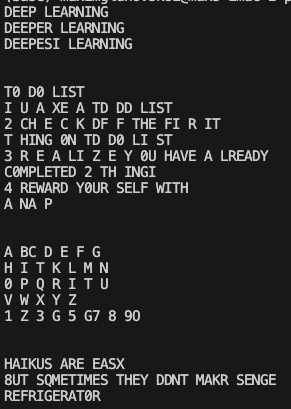
\includegraphics[width=0.6\linewidth]{final_res2.png}
\end{figure}

\end{document}